\section{More Simulation Results}\label{appendix: more_result}

\begin{figure}[H] 
\centering 
    \centering 
    \begin{subfigure}{0.32\textwidth}
    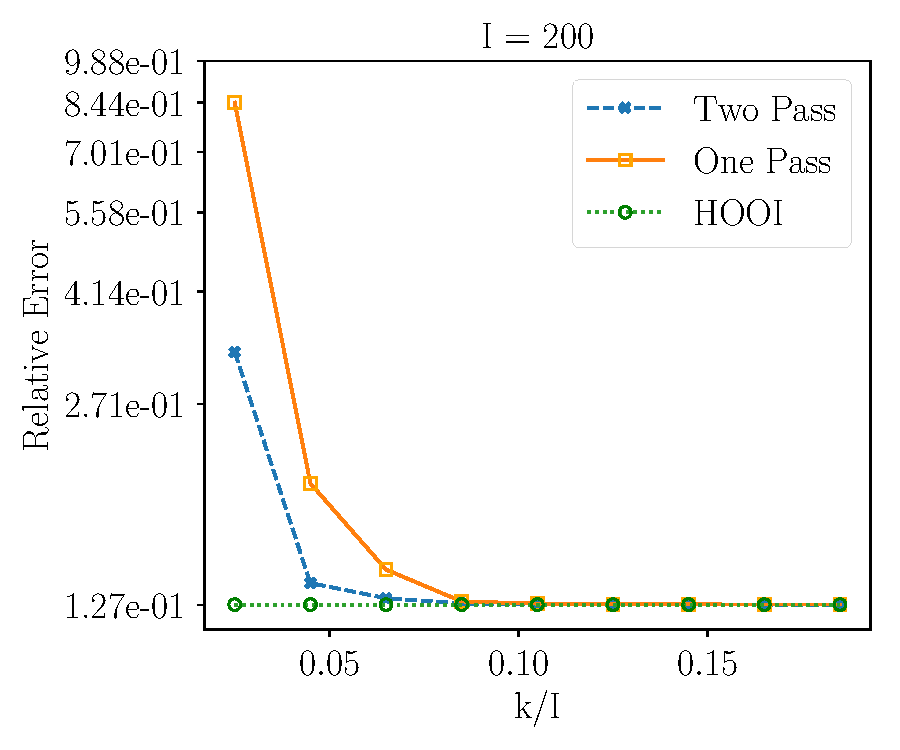
\includegraphics[scale = 0.3]{figure/fpd_n200.pdf}
    \end{subfigure}
    \begin{subfigure}{0.32\textwidth}
    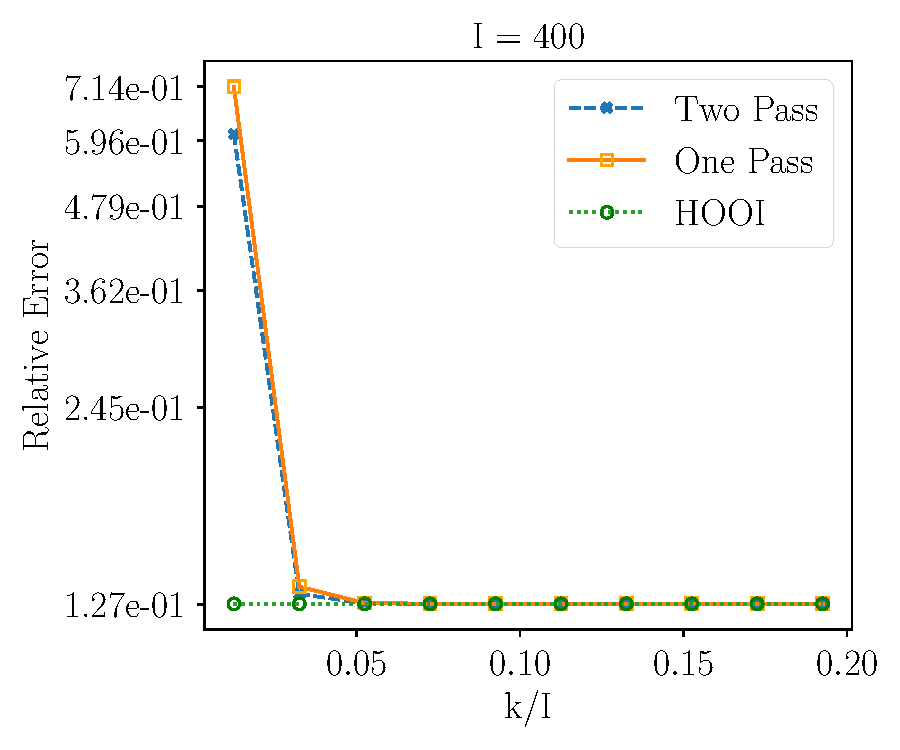
\includegraphics[scale = 0.3]{figure/fpd_n400.pdf}
    \end{subfigure}
    \begin{subfigure}{0.32\textwidth}
    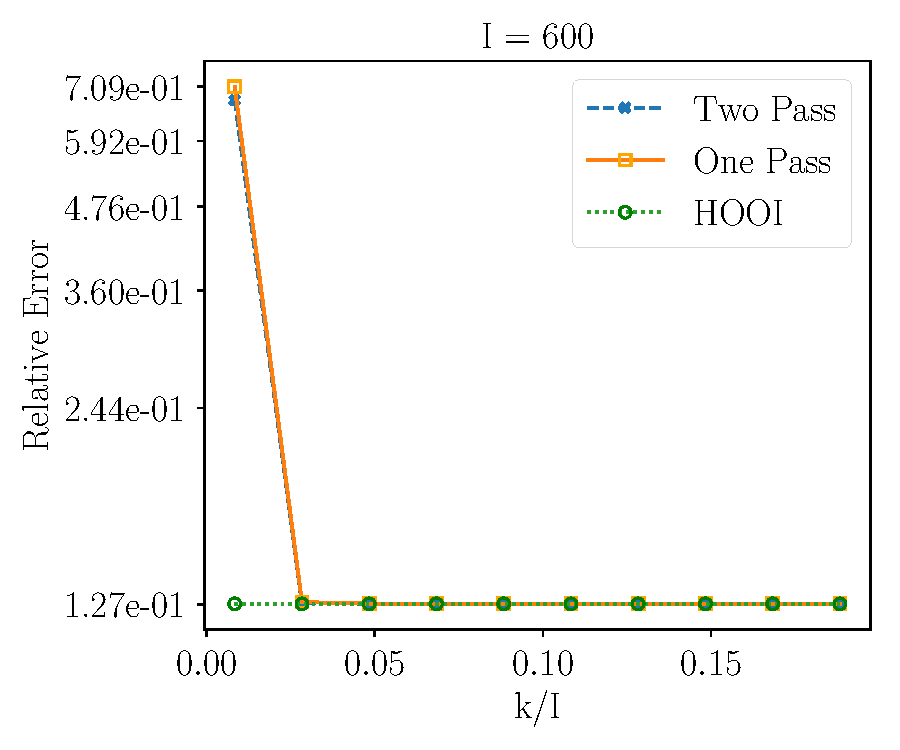
\includegraphics[scale = 0.3]{figure/fpd_n600.pdf}
    \end{subfigure}
\textbf{Superdiagonal + Low Noise ($\gamma = 0.01, \, r = 1$)}\\
    \centering 
    \begin{subfigure}{0.32\textwidth}
    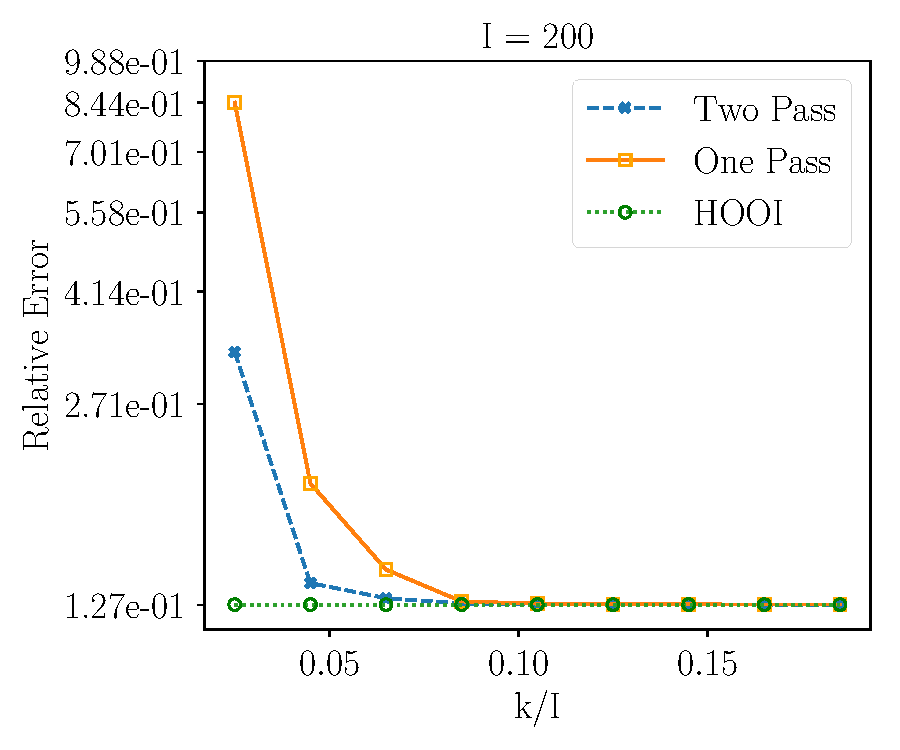
\includegraphics[scale = 0.3]{figure/fpd_n200.pdf}
    \end{subfigure}
    \begin{subfigure}{0.32\textwidth}
    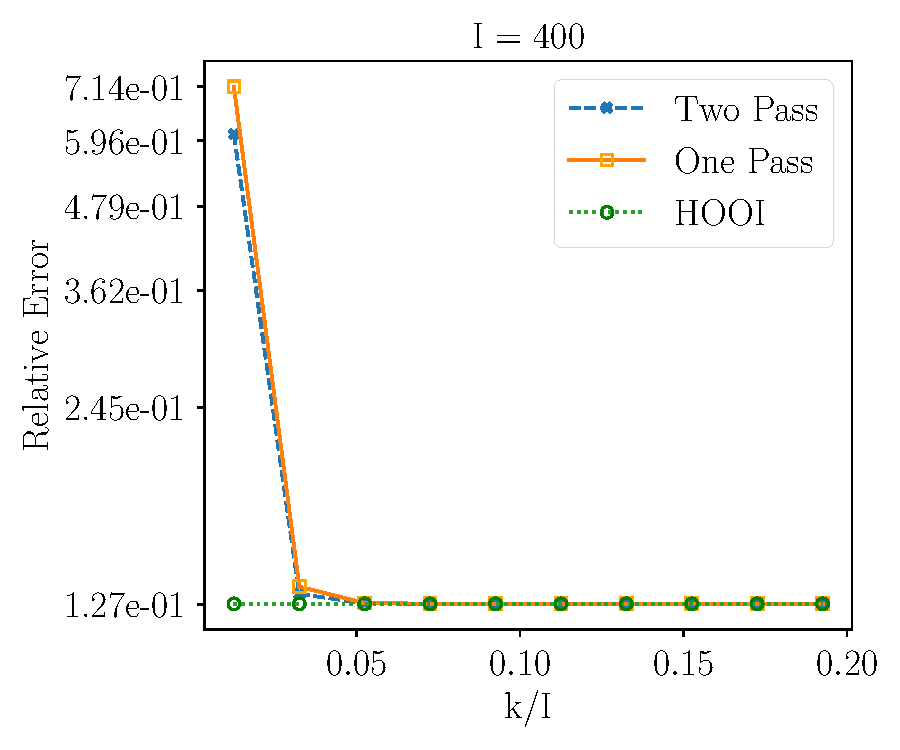
\includegraphics[scale = 0.3]{figure/fpd_n400.pdf}
    \end{subfigure}
    \begin{subfigure}{0.32\textwidth}
    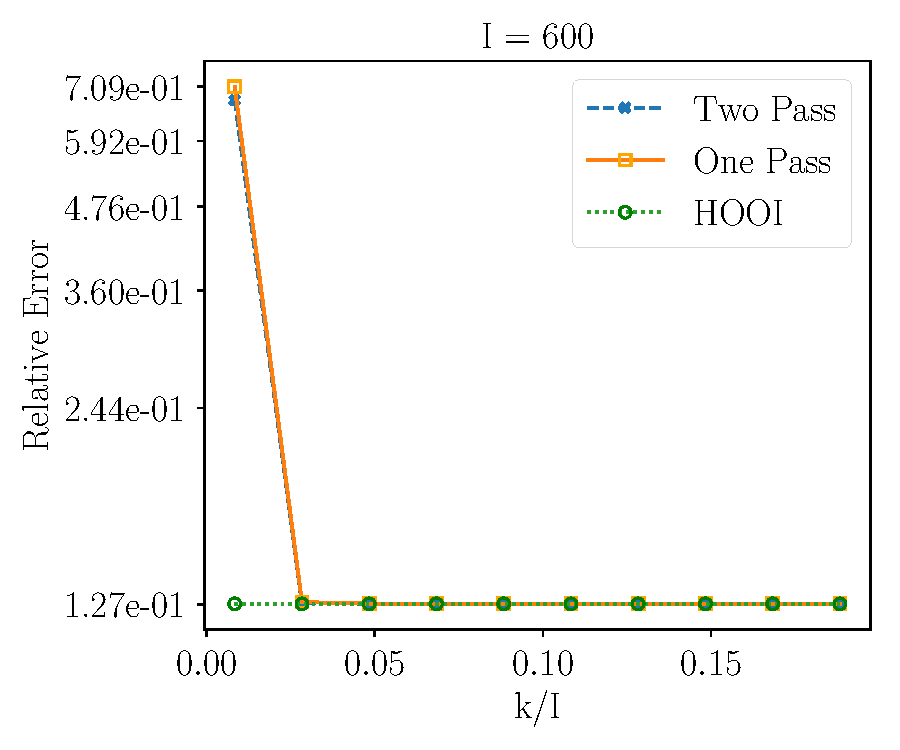
\includegraphics[scale = 0.3]{figure/fpd_n600.pdf}
    \end{subfigure}
\textbf{Fast Polynomial Decay ($t = 2$)}\\
    \centering 
    \begin{subfigure}{0.32\textwidth}
    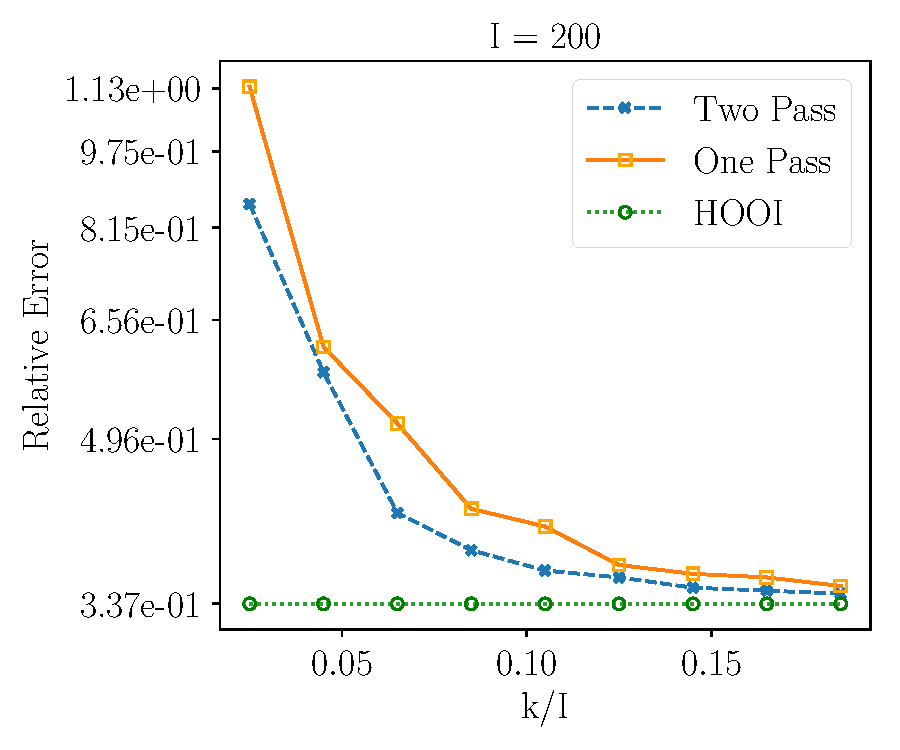
\includegraphics[scale = 0.3]{figure/spd_n200.pdf}
    \end{subfigure}
    \begin{subfigure}{0.32\textwidth}
    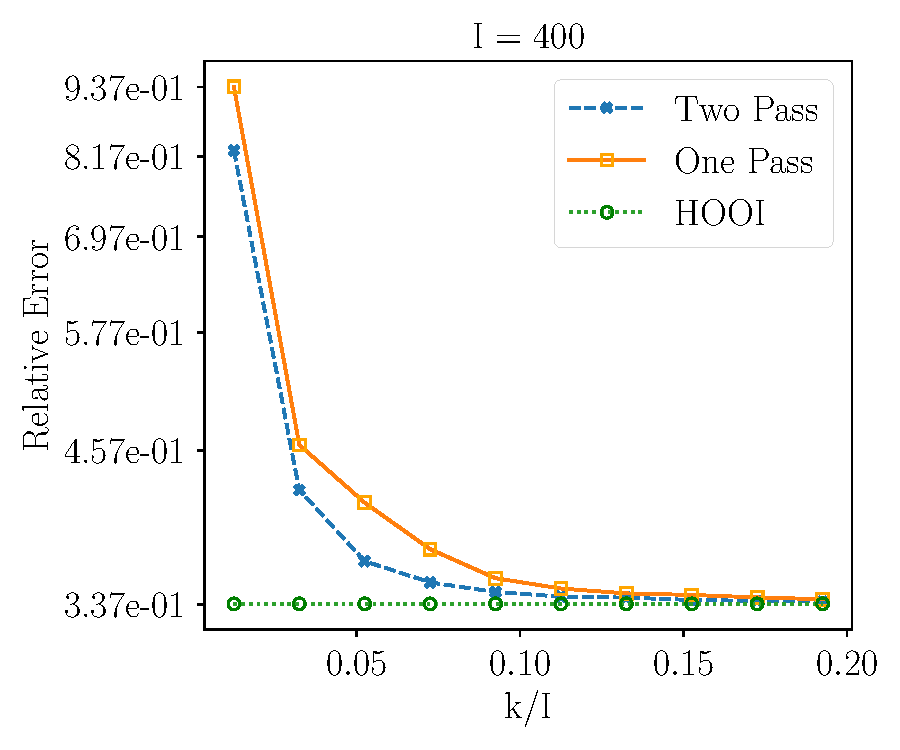
\includegraphics[scale = 0.3]{figure/spd_n400.pdf}
    \end{subfigure}
    \begin{subfigure}{0.32\textwidth}
    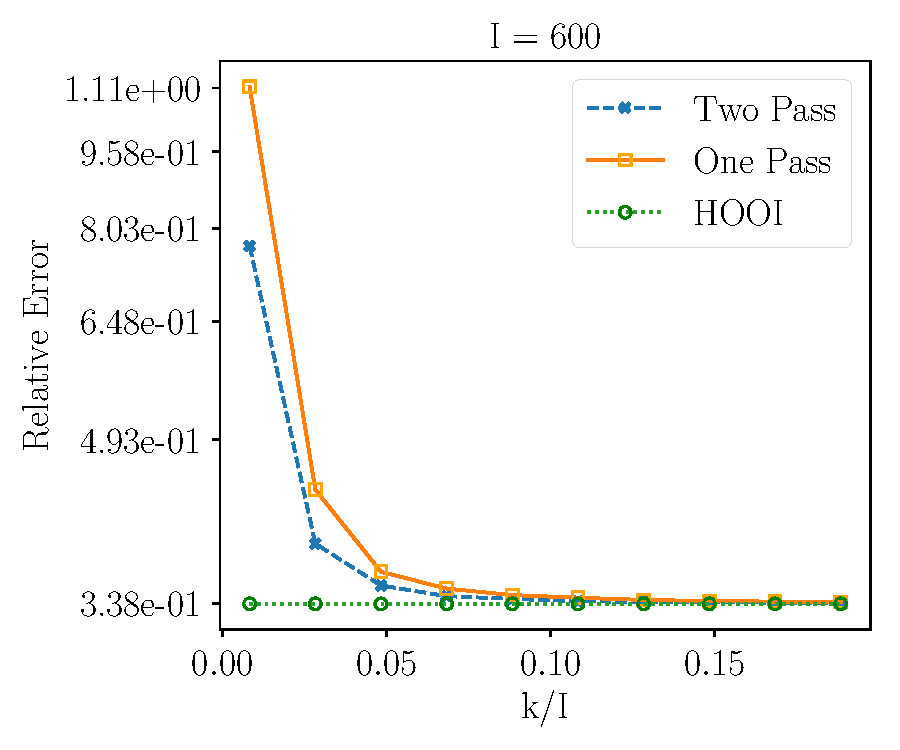
\includegraphics[scale = 0.3]{figure/spd_n600.pdf}
    \end{subfigure}
\textbf{Slow Polynomial Decay ($t = 1$)}\\
    \centering 
    \begin{subfigure}{0.32\textwidth}
    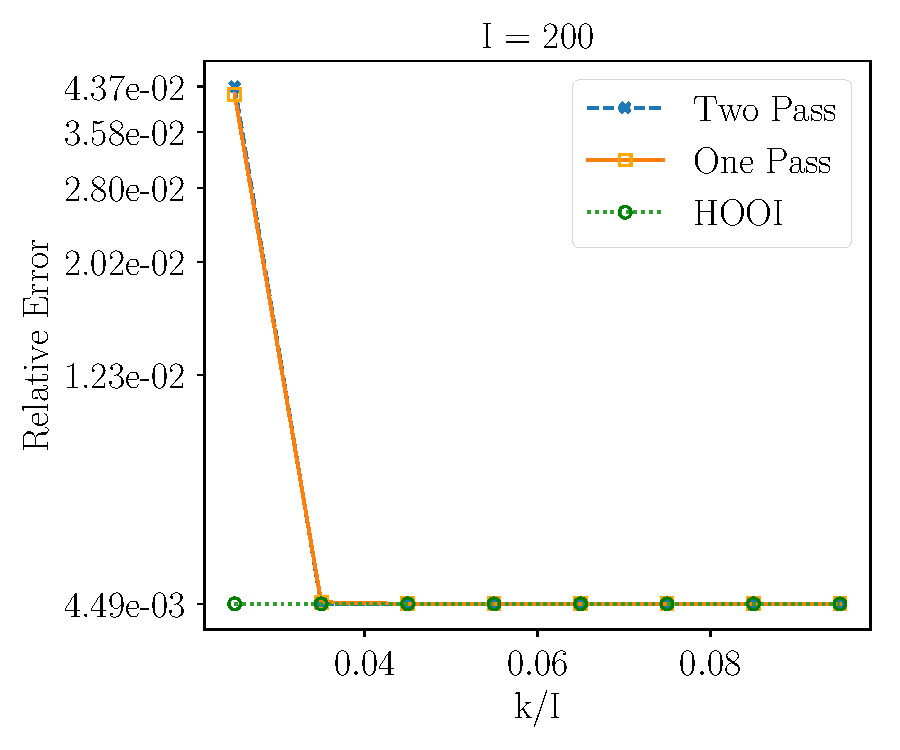
\includegraphics[scale = 0.3]{figure/fed_n200.pdf}
    \end{subfigure}
    \begin{subfigure}{0.32\textwidth}
    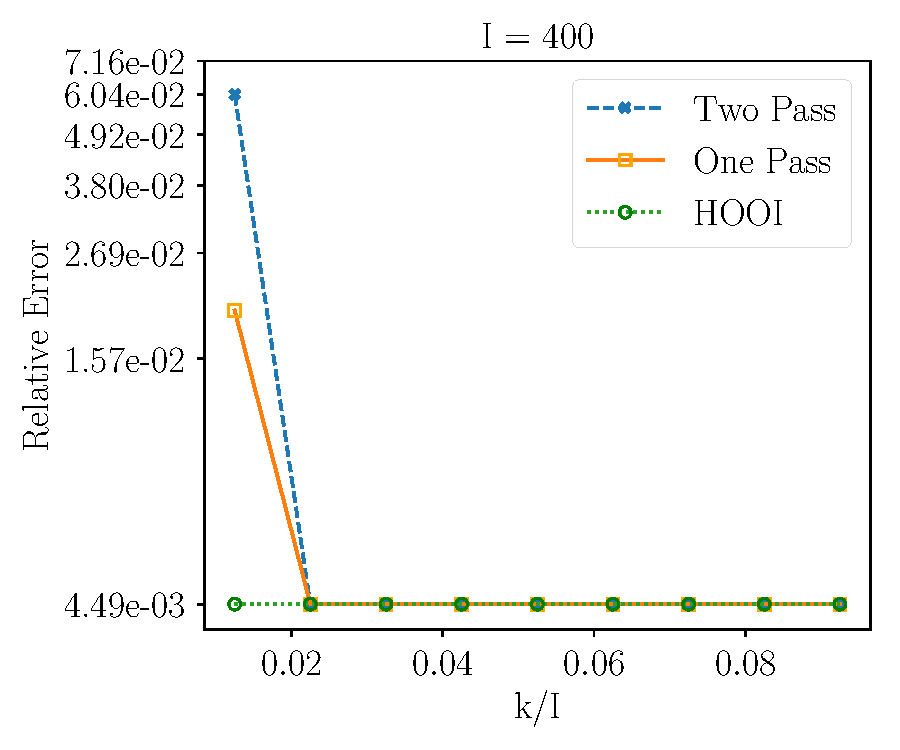
\includegraphics[scale = 0.3]{figure/fed_n400.pdf}
    \end{subfigure}
    \begin{subfigure}{0.32\textwidth}
    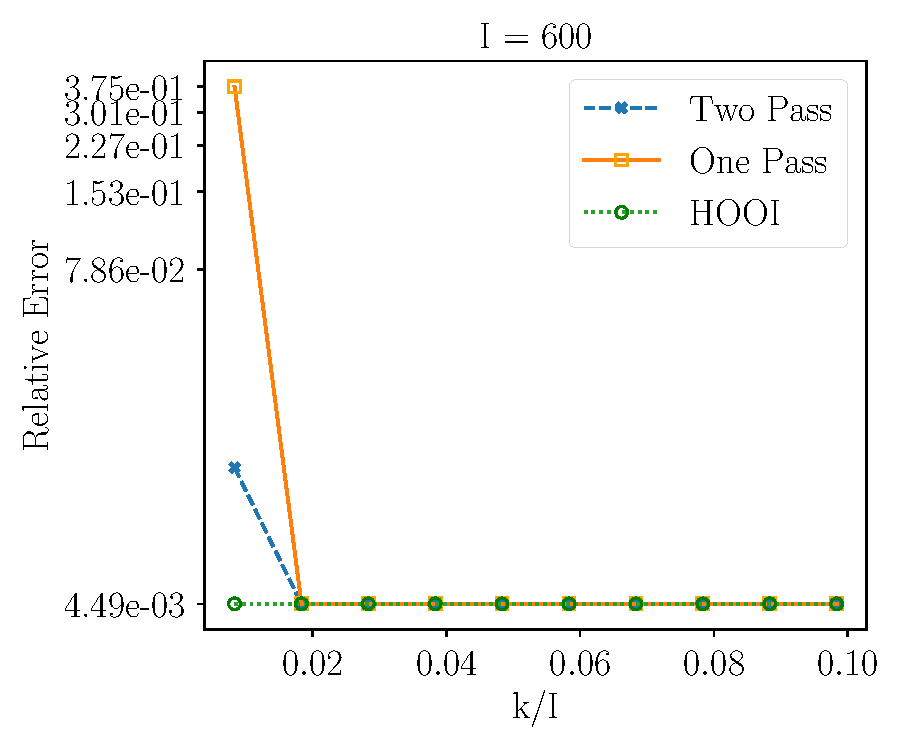
\includegraphics[scale = 0.3]{figure/fed_n600.pdf}
    \end{subfigure}
\textbf{Fast Exponential Decay ($t = 1$)}\\
    \centering 
    \begin{subfigure}{0.32\textwidth}
    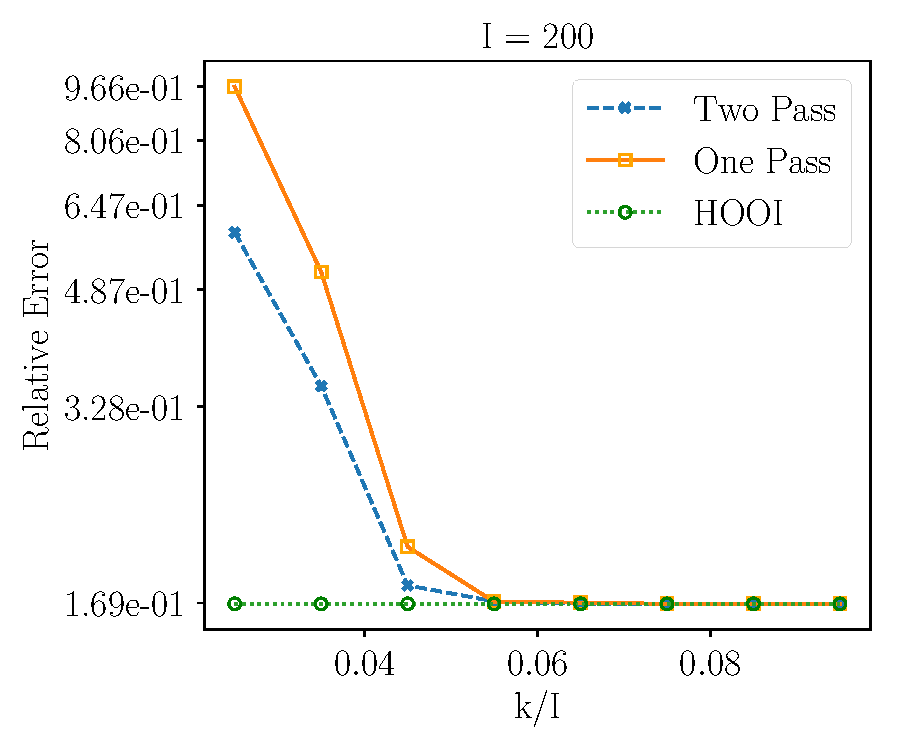
\includegraphics[scale = 0.3]{figure/sed_n200.pdf}
    \end{subfigure}
    \begin{subfigure}{0.32\textwidth}
    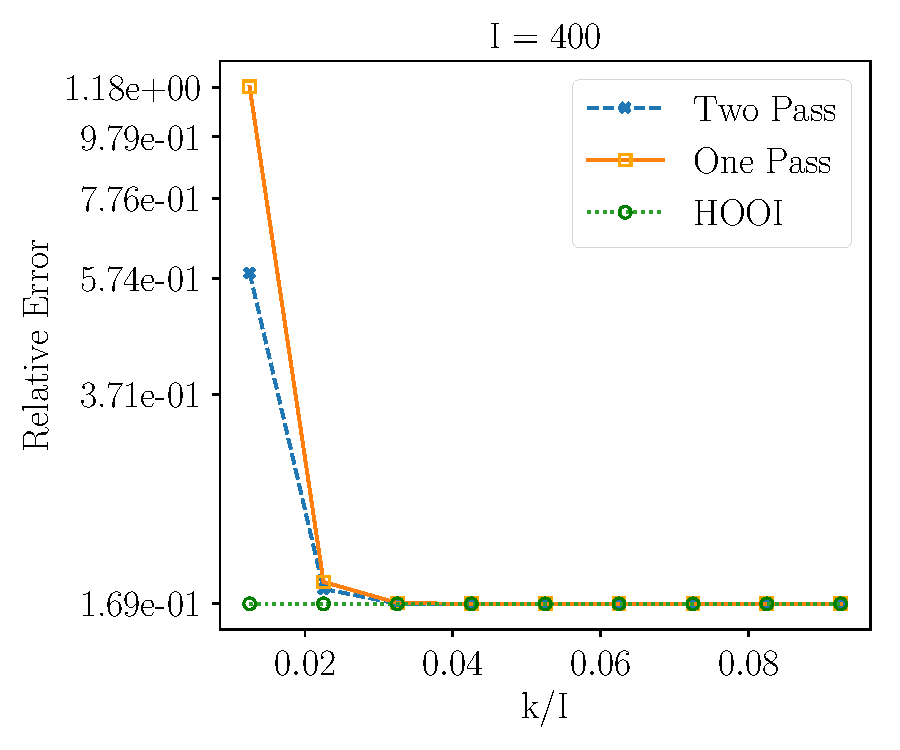
\includegraphics[scale = 0.3]{figure/sed_n400.pdf}
    \end{subfigure}
    \begin{subfigure}{0.32\textwidth}
    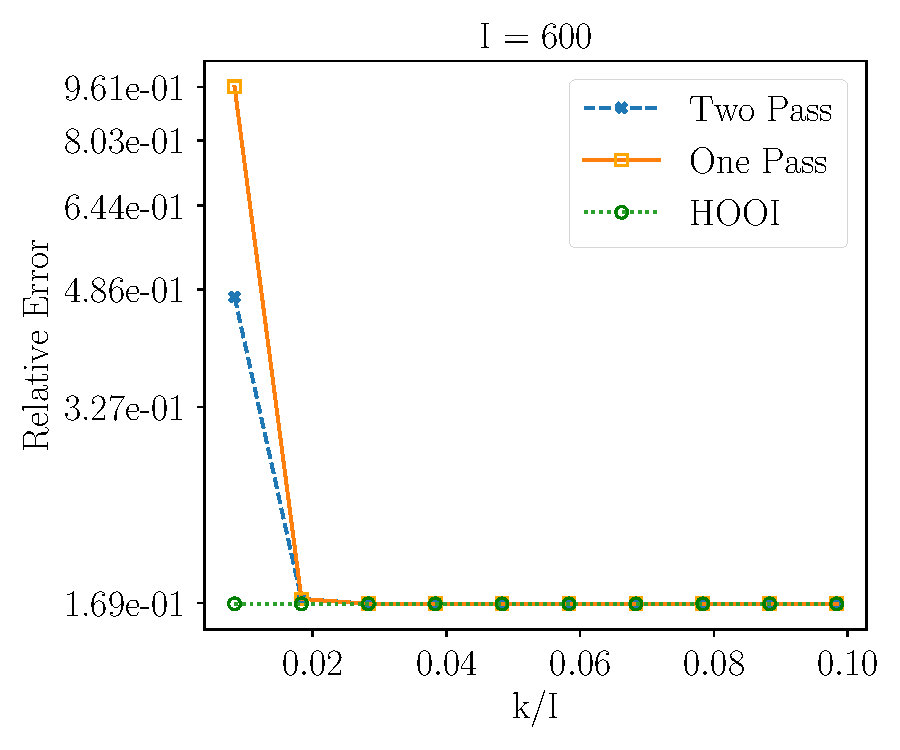
\includegraphics[scale = 0.3]{figure/sed_n600.pdf}
    \end{subfigure}
\textbf{Slow Exponential Decay ($t = 0.25$)} \\ 
\captionsetup{labelformat=empty}
\end{figure}

\setcounter{figure}{2}    
\begin{figure}[H]
\centering
    \begin{subfigure}{0.32\textwidth}
    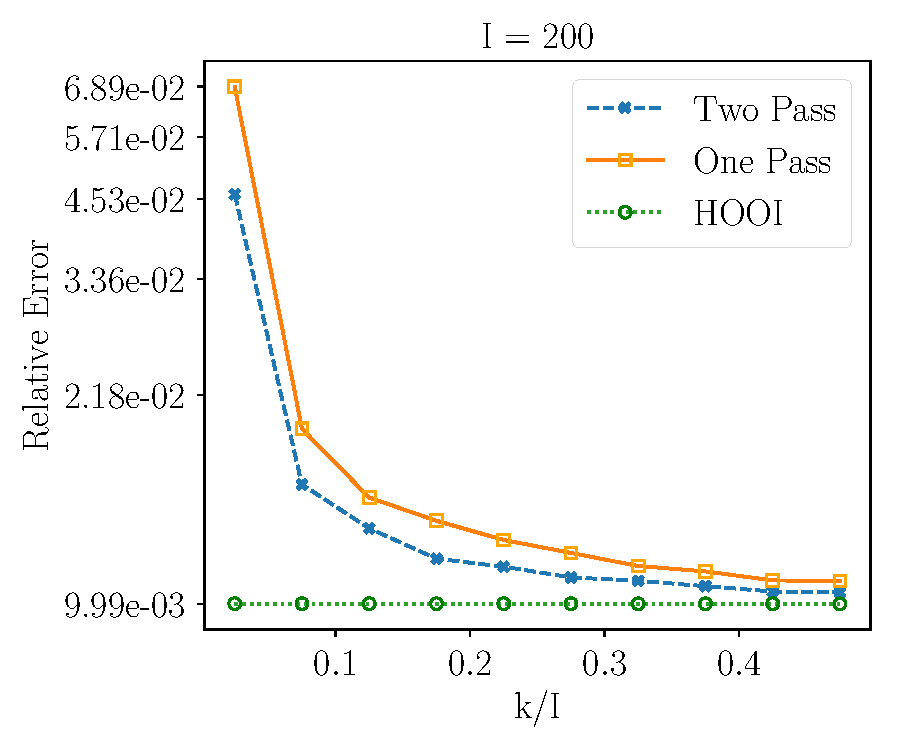
\includegraphics[scale = 0.3]{figure/lk_lnoise_n200.pdf}
    \end{subfigure}
    \begin{subfigure}{0.32\textwidth}
    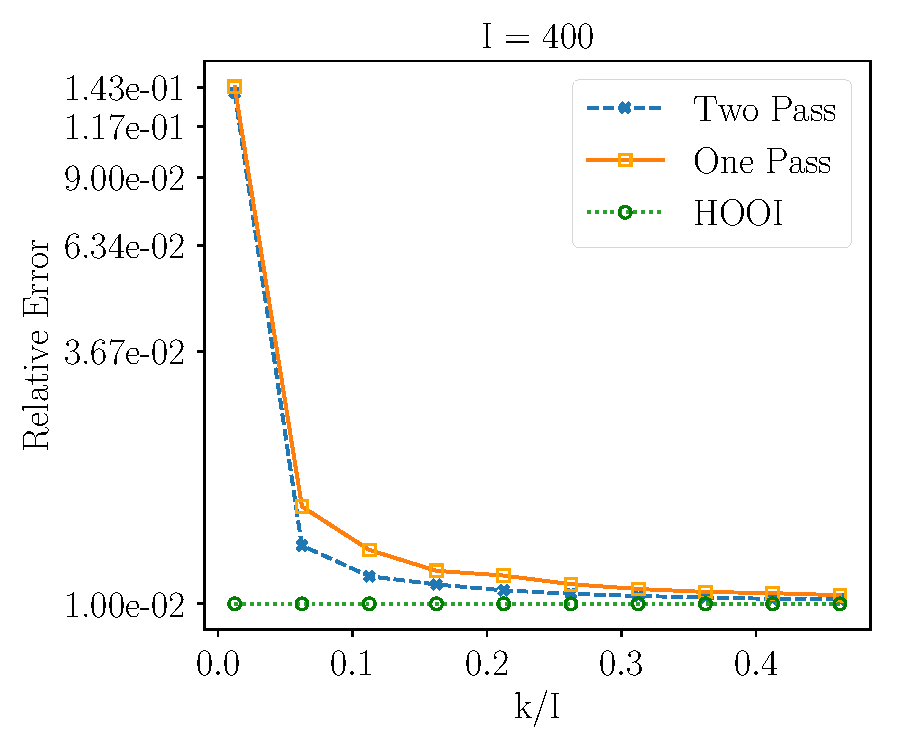
\includegraphics[scale = 0.3]{figure/lk_lnoise_n400.pdf}
    \end{subfigure}
    \begin{subfigure}{0.32\textwidth}
    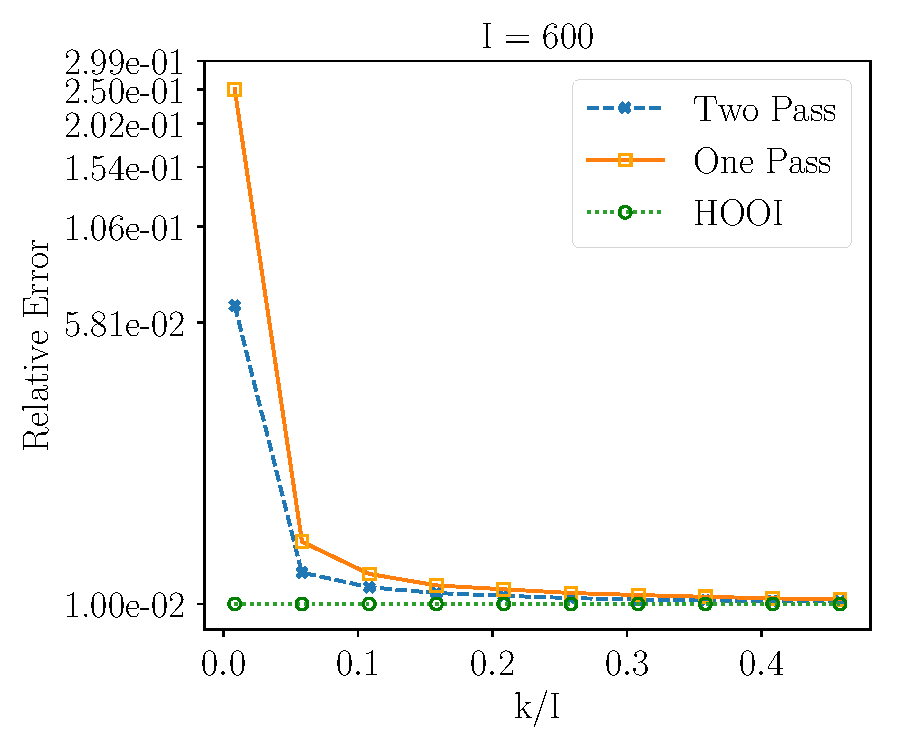
\includegraphics[scale = 0.3]{figure/lk_lnoise_n600.pdf}
    \end{subfigure}
\textbf{Low Rank + Low Noise ($\gamma = 0.01$)} \\ 
\centering
    \begin{subfigure}{0.32\textwidth}
    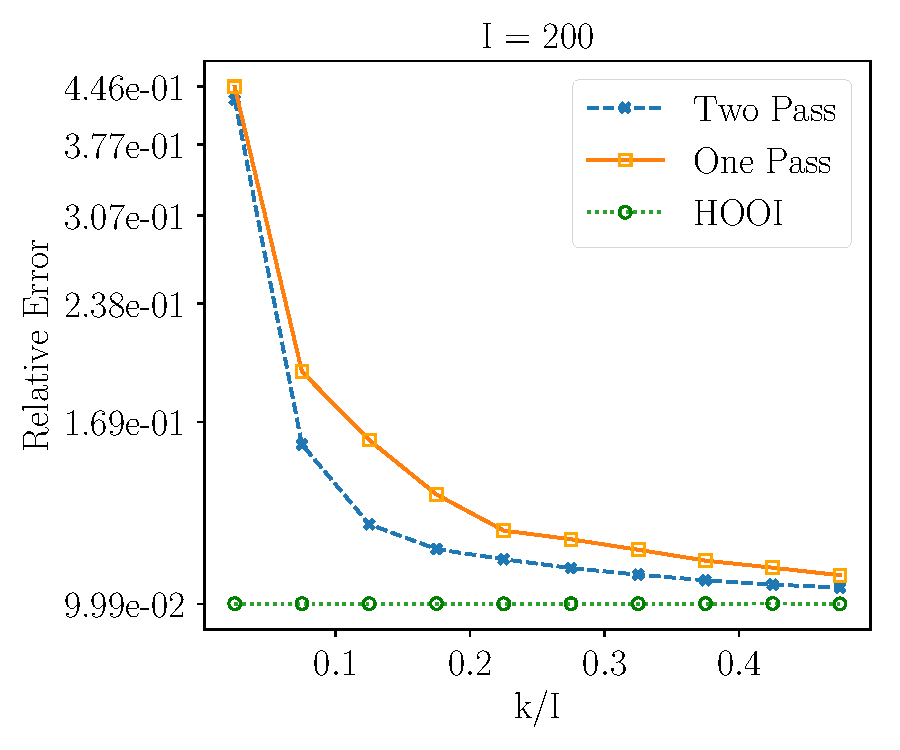
\includegraphics[scale = 0.3]{figure/lk_mnoise_n200.pdf}
    \end{subfigure}
    \begin{subfigure}{0.32\textwidth}
    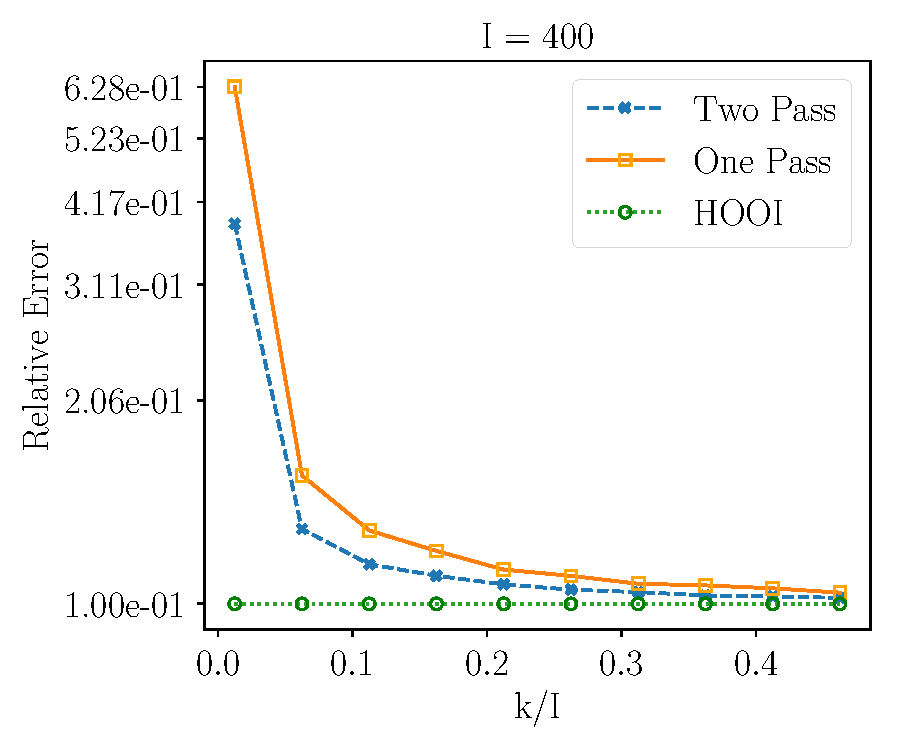
\includegraphics[scale = 0.3]{figure/lk_mnoise_n400.pdf}
    \end{subfigure}
    \begin{subfigure}{0.32\textwidth}
    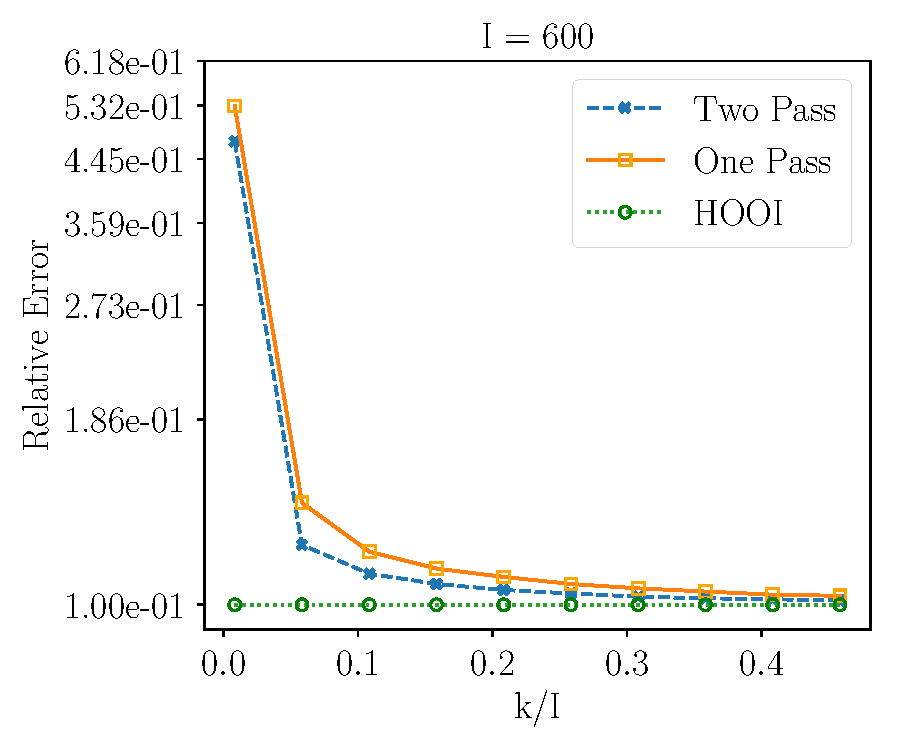
\includegraphics[scale = 0.3]{figure/lk_mnoise_n600.pdf}
    \end{subfigure}
\textbf{Low Rank + Medium Noise ($\gamma = 0.1$)} \\ 
    \begin{subfigure}{0.32\textwidth}
    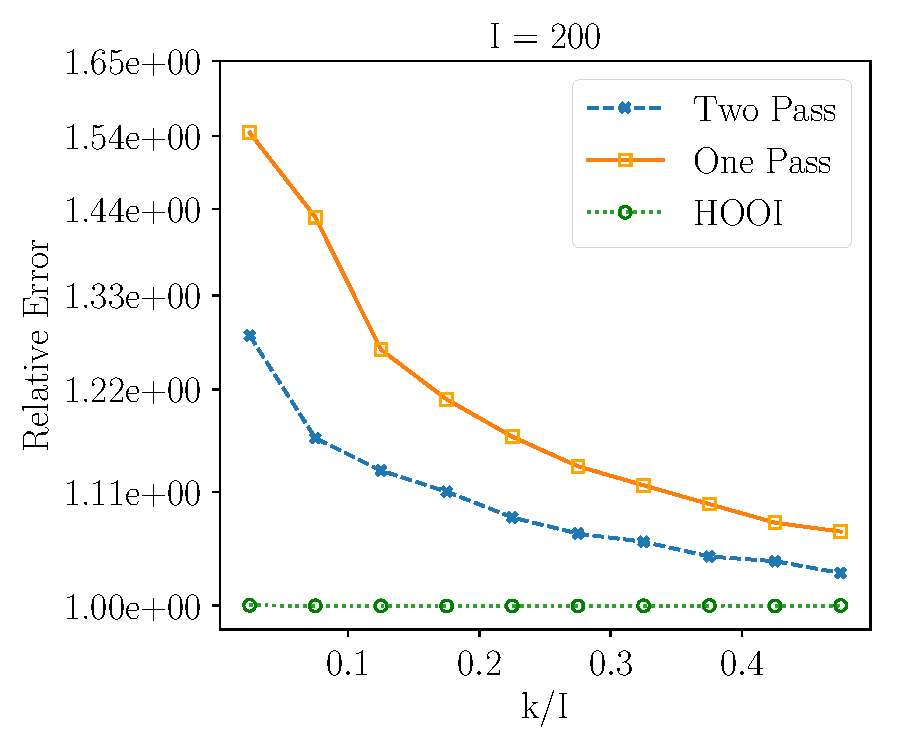
\includegraphics[scale = 0.3]{figure/lk_hnoise_n200.pdf}
    \end{subfigure}
    \begin{subfigure}{0.32\textwidth}
    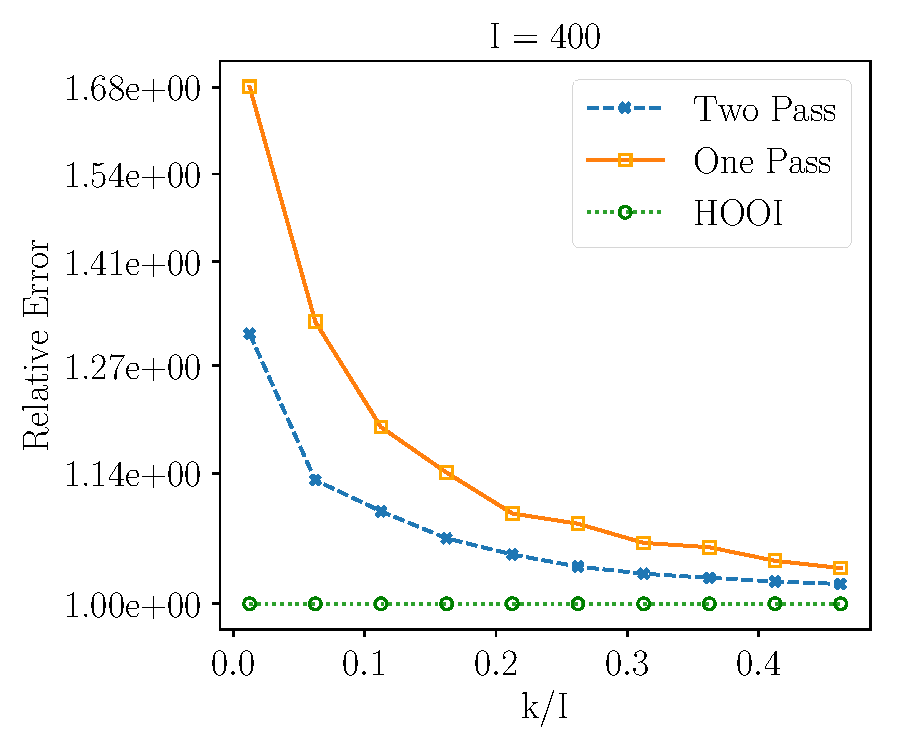
\includegraphics[scale = 0.3]{figure/lk_hnoise_n400.pdf}
    \end{subfigure}
    \begin{subfigure}{0.32\textwidth}
    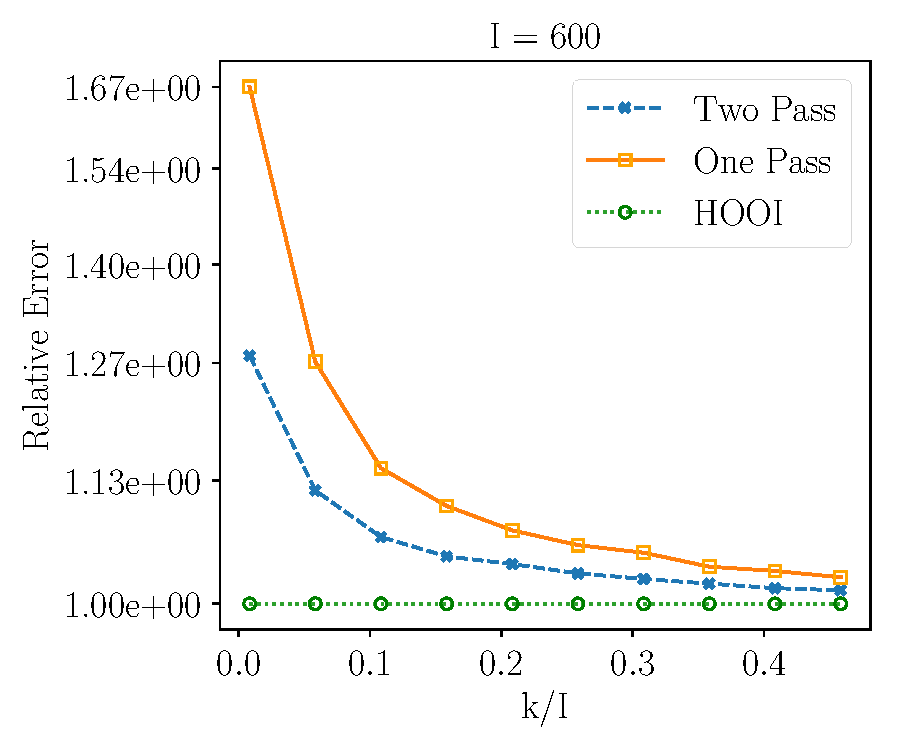
\includegraphics[scale = 0.3]{figure/lk_hnoise_n600.pdf}
    \end{subfigure}
\textbf{Low Rank + High Noise ($\gamma = 1$)} \\ 

\caption{Relative error for fixed-rank tensor approximation as a function of the compression factor $k/n$: \textit{We compare the relative error presented in log scale for two-pass sketching, one-pass sketching and Tucker decomposition for different design tensors when n = 200, 400, 600. $r = 5$ except for the first row.}} \label{fig:more_result}
\end{figure}

